\documentclass{article}
\usepackage{amsmath}
\usepackage{amssymb}
\usepackage[a4paper, top=25mm, bottom=25mm, left=25mm, right=25mm]{geometry}
\usepackage{pgfplots}
\usepackage{mathtools}
\pgfplotsset{compat=1.18}
\usepgfplotslibrary{fillbetween}

\begin{document}
\pagestyle{empty}
\large

\begin{center}
2014-2015 Summer \\MAT123 Final\\(23/08/2015)
\end{center}

\noindent 1. Sketch the graph of $f(x)=\ln\left(x^2+1\right)$.

\hfill

\noindent 2. Determine the area of the region bounded by $y=4x+3$ and $y=6-x-2x^2$.

\hfill

\noindent 3. Use the Washer Method to find the volume of the solid obtained by revolving the region bounded by $y=2\sqrt{x-1},\: y=x-1$ about the line $x=-1$, respectively.

\hfill

\noindent 4. Use the Cylindrical Shell Method to find the volume of the solid obtained by revolving the region bounded by $x=y^2-4$ and $x=6-3y$ about $y=-8$.

\hfill

\noindent 5. Evaluate the following integrals.

\hfill

(a) $\displaystyle\int4\left(\frac1x-\mathrm{e}^{-x}\right)\cos\left(\mathrm{e}^{-x}+\ln x\right)\,dx$

\hfill

\hfill

(b) $\displaystyle\int\frac{x^3+10x^2+3x+36}{(x-1)^2\,\left(x^2+4\right)^2}\,dx$

\hfill

\hfill

(c) $\displaystyle\int\frac{\sqrt{25x^2-4}}{x}\,dx$

\hfill

\hfill

(d) $\displaystyle\int x^2\cos(4x)\,dx$

\hfill

\hfill

(e) $\displaystyle\int\frac{dx}{2x^2-3x+2}$

\hfill

\noindent 6. Investigate the convergence of the improper integral $\displaystyle\int_{-\infty}^0(1+2x)\,\mathrm{e}^{-x}\,dx$.

\hfill

\noindent 7. Evaluate the arc length $\displaystyle x=\frac23(y-1)^{3/2}$ for $1\leq y\leq2$.

\newpage

\begin{center}
2014-2015 Summer Final (23/08/2015) Solutions\\
(Last update: 20/10/2025 23:04)
\end{center}

\noindent 1. $\ln x$ is defined for $x>0$. Therefore, $\ln\left(x^2+1\right)$ is defined on $\mathbb{R}$ because $x^2+1\geq1>0$.

\hfill

\noindent Let us find the limit at infinity and negative infinity.

\begin{equation*}\lim_{x\to\infty}\ln\left(x^2+1\right)=\lim_{x\to-\infty}\ln\left(x^2+1\right)=\infty\end{equation*}

\hfill

\noindent No asymptotes occur.

\hfill

\noindent Take the first derivative and find the critical points. Apply the chain rule.

\[y'=\frac d{dx}\ln\left(x^2+1\right)=\frac1{x^2+1}\cdot 2x=\frac{2x}{x^2+1}\]

\hfill

\noindent A critical point occurs at $x=0$. At this point, the first derivative is $0$.

\hfill

\noindent Take the second derivative. Apply the quotient rule.

\[y''=\frac d{dx}\left(\frac{2x}{x^2+1}\right)=\frac{2\cdot\left(x^2+1\right)-2x\cdot(2x)}{\left(x^2+1\right)^2}=\frac{2-2x^2}{\left(x^2+1\right)^2}\]

\hfill

\noindent The inflection points occur at $x=\pm1$. At these points, the direction of the curvature changes.

\hfill

\noindent Consider some values of the function. Eventually, set up a table and see what the graph looks like in certain intervals.

\begin{equation*}\,f\left(-1\right)=f\left(1\right)=\ln2,\quad f(0)=0\end{equation*}

\begin{center}
    \large
    \begin{tabular}{|c|cccc|} 
    \hline
        $x$&$\left(-\infty,-1\right)$&$\left(-1,0\right)$&$\left(0,1\right)$&$\left(1, \infty\right)$\\
        \hline
        $y$&$(\ln2,\infty)$&$(0,\ln2)$&$(0,\ln2)$&$(\ln2,\infty)$\\
        \hline
        $y'$ sign&-&-&+&+\\
        \hline
        $y''$ sign&-&+&+&-\\
        \hline
    \end{tabular}
\end{center}

\hfill

\begin{center}
\begin{tikzpicture}
  \begin{axis}[
    axis lines = center,
    xlabel = $x$, ylabel = $y$,
    domain=-4:4,
    samples=200,
    ymin=0, ymax=3,
    xmin=-3, xmax=3,
    restrict y to domain=-5:5,
    enlargelimits=true,
    axis line style={->},
    scale=1.4,
    ]
    \addplot[blue, thick] {ln(x^2+1)};
    \draw[dashed](-1,0)--(-1,0.693);\draw[dashed](1,0)--(1,0.693);\draw[dashed](-1,0.693)--(0,0.693);\draw[dashed](0,0.693)--(1,0.693);
    \node at (-0.2,0.77) {\small$\ln2$};
  \end{axis}
\end{tikzpicture}
\end{center}

\newpage

\noindent 2.
\begin{center}
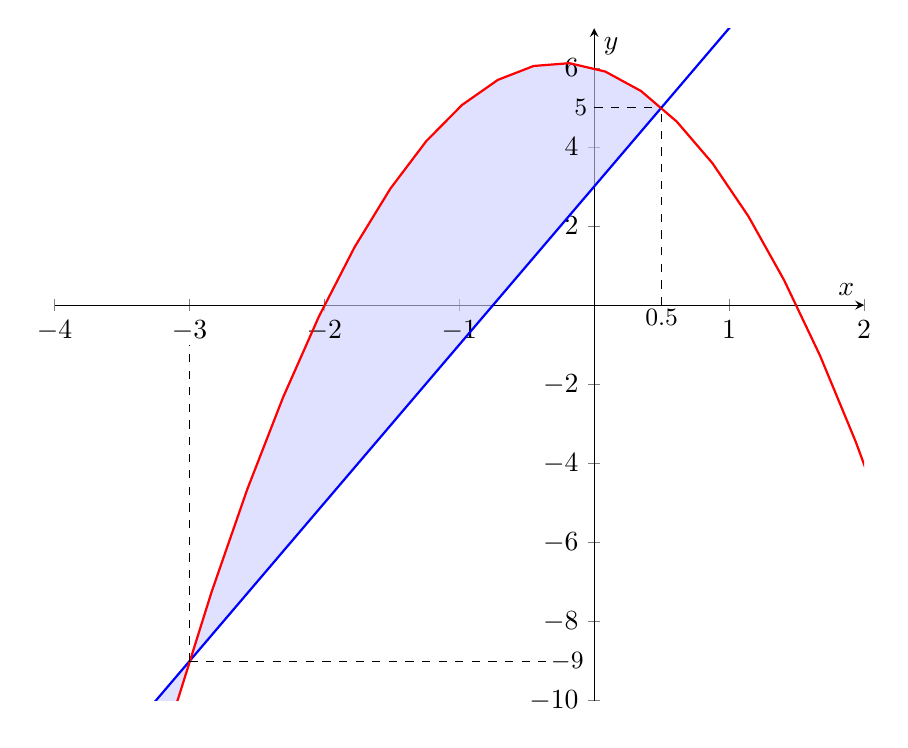
\begin{tikzpicture}
  \begin{axis}[
      axis lines=center,
      xlabel={$x$},
      ylabel={$y$},
      xmin=-4, xmax=2,
      ymin=-10, ymax=7,
      samples=50,
      clip=true,
      scale=1.5,
      domain=-10:3,
    ]

    \addplot [thick, blue, name path=A] {4*x+3};
    \addplot [thick, red, domain=-10:3, name path=B] {6-x-2*x^2};
    \addplot [blue!20, fill opacity=0.6] fill between[of=A and B,soft clip={domain=-9:0.5}];
    
    \draw[dashed] (-3,-9) -- (-3,-1); \draw[dashed] (-3,-9) -- (-0.3,-9);
    \draw[dashed] (0.5,0) -- (0.5,5); \draw[dashed] (0,5) -- (0.5,5);

    \node at (axis cs:-0.1,5) {\small $5$};
    \node at (axis cs:-0.2,-9) {\small $-9$};
    \node at (axis cs:0.5,-0.3) {\small $0.5$};
  \end{axis}
\end{tikzpicture}
\end{center}
\begin{align*}
\text{Area}&=\int_{-3}^{1/2}\left[6-x-2x^2-(4x+3)\right]\,dx=\int_{-3}^{1/2}\left(3-5x-2x^2\right)\,dx\\\\&=3x-\frac{5x^2}2-\frac{2x^3}3\Bigg|_{-3}^{1/2}=\left(\frac32-\frac58-\frac1{12}\right)-\left(-9-\frac{45}2+18\right)=\boxed{\frac{343}{24}}
\end{align*}

\hfill

\noindent 3.
\begin{center}
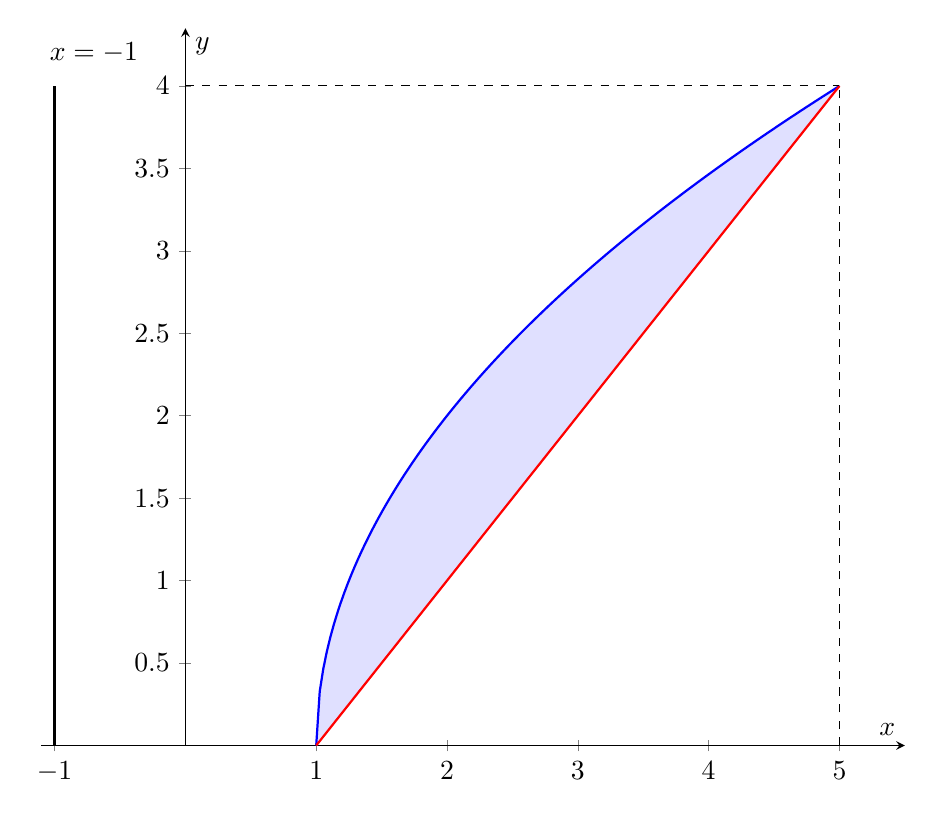
\begin{tikzpicture}
  \begin{axis}[
      axis lines=center,
      xlabel={$x$},
      ylabel={$y$},
      xmin=-1.1, xmax=5.5,
      ymin=0, ymax=4.35,
      samples=150,
      clip=true,
      scale=1.6,
      domain=1:5,
    ]

    \addplot [thick, blue, name path=A] {2*sqrt(x-1)};
    \addplot [thick, red, name path=B] {x-1};
    \addplot [blue!20, fill opacity=0.6] fill between[of=A and B,soft clip={domain=1:5}];
    
    \draw[dashed] (5,0) -- (5,4); \draw[thick] (-1,0) -- (-1,4); \draw[dashed] (0,4) -- (5,4);
    \node at (-0.7,4.2) {$x=-1$};
  \end{axis}
\end{tikzpicture}
\end{center}

\noindent Rewrite the equations of the curves and solve for $x$. Let $V$ be the volume of the solid.

\[y=2\sqrt{x-1}\implies y^2=4x-4\implies x=\frac{y^2+4}4\]
\[y=x-1\implies x=y+1\]

\begin{align*}
V&=\int_D\pi\left[R_2^2(y)-R_1^2(y)\right]\,dy=\int_0^4\pi\left[\left((y+1)+1\right)^2-\left(\left(\frac{y^2+4}4\right)+1\right)^2\right]\,dy\\\\&=\pi\int_0^4\left[(y+2)^2-\left(\frac{y^2}4+2\right)^2\right]\,dy=\pi\int_0^4\left(y^2+4y+4-\frac{y^4}{16}-y^2-4\right)\,dy\\\\&=\pi\int_0^4\left(4y-\frac{y^4}{16}\right)\,dy=\pi\left[2y^2-\frac{y^5}{80}\right]_0^4=\pi\left[\left(32-\frac{64}{5}\right)-\left(0\right)\right]=\boxed{\frac{96\pi}5}
\end{align*}

\hfill

\noindent 4.
\begin{center}
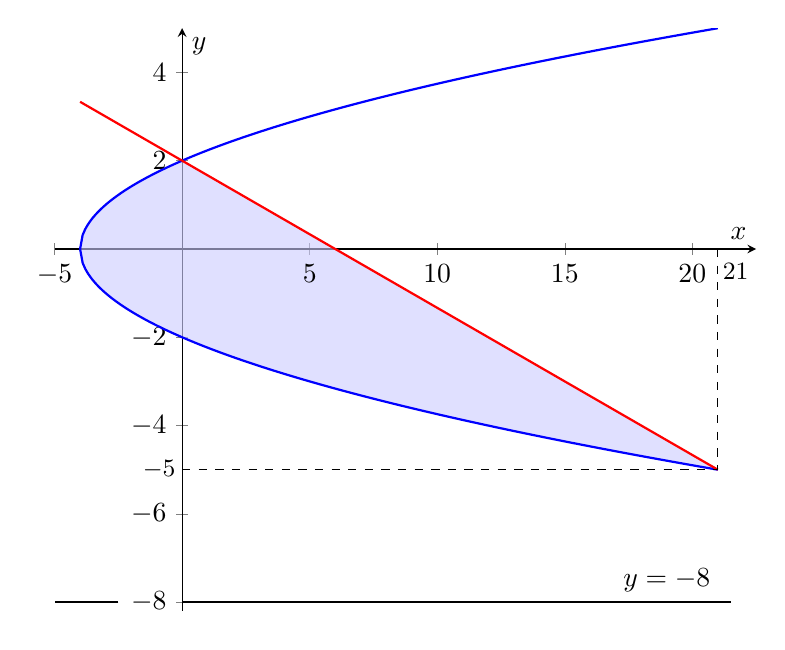
\begin{tikzpicture}
  \begin{axis}[
      axis lines=center,
      xlabel={$x$},
      ylabel={$y$},
      xmin=-5, xmax=22.5,
      ymin=-8.2, ymax=5,
      samples=250,
      clip=true,
      scale=1.3,
      domain=-4:21,
    ]

    \addplot [thick, blue, name path=A] {sqrt(x+4)};
    \addplot [thick, blue, name path=B] {-sqrt(x+4)};
    \addplot [thick, red, name path=C] {(6-x)/3};
    \addplot [blue!20, fill opacity=0.6] fill between[of=A and B,soft clip={domain=-4:0}];
    \addplot [blue!20, fill opacity=0.6] fill between[of=C and B,soft clip={domain=0:21}];

    \draw[dashed] (21,0)--(21,-5); \draw[thick] (0,-8)--(21.5,-8); \draw[thick] (-2.5,-8)--(-5,-8); \draw[dashed] (0,-5)--(21,-5);
    \node at (19,-7.5) {$y=-8$};
    \node at (21.7,-0.5) {\small $21$};
    \node at (-0.9,-5) {\small $-5$};
  \end{axis}
\end{tikzpicture}
\end{center}

\noindent Let $V$ be the volume of the solid.

\begin{align*}
V&=\int_D2\pi\cdot h(y)\cdot r(y)\,dy=2\pi\int_{-5}^2(y+8)\cdot\left[(6-3y)-(y^2-4)\right]\,dy\\\\&=2\pi\int_{-5}^2(y+8)(-y^2-3y+10)\,dy=2\pi\int_{-5}^2\left(-y^3-3y^2+10y-8y^2-24y+80\right)\,dy\\\\&=2\pi\int_{-5}^2\left(-y^3-11y^2-14y+80\right)\,dy=2\pi\left[-\frac{y^4}4-\frac{11y^3}3-7y^2+80y\right]_{-5}^2\\\\&=2\pi\left[\left(-4-\frac{88}3-28+160\right)-\left(\frac{625}4+\frac{1375}3-175-400\right)\right]=\boxed{\frac{4459\pi}6}
\end{align*}

\newpage

\noindent 5.

\hfill

\noindent (a) Use the $u$-substitution method. Let $u=\mathrm{e}^{-x}+\ln x$. Then $\displaystyle du=\left(-\mathrm{e}^{-x}+\frac1x\right)\,dx$.

\begin{align*}\int4\left(\frac1x-\mathrm{e}^{-x}\right)\cos\left(\mathrm{e}^{-x}+\ln x\right)\,dx&=\int4\cos u\,du=4\sin u+c\\\\&=\boxed{4\sin\left(\mathrm{e}^{-x}+\ln x\right)+c,\:c\in\mathbb{R}}\end{align*}

\hfill

\noindent (b) Decompose the fraction into multiple partial fractions. Let $A,\:B,\:C,\:D,\:E,\:F\in\mathbb{R}$.

\begin{align*}\mathrm{I}=\int\frac{x^3+10x^2+3x+36}{(x-1)^2\,\left(x^2+4\right)^2}\,dx=\int\left(\frac{A}{x-1}+\frac{B}{(x-1)^2}+\frac{Cx+D}{x^2+4}+\frac{Ex+F}{(x^2+4)^2}\right)\,dx\end{align*}

\hfill

\noindent Let $N=x^3+10x^2+3x+36$.

\begin{align*}
N&=A\left(x^2+4\right)^2(x-1)+B\left(x^2+4\right)^2+(Cx+D)\left(x^2+4\right)(x-1)^2+(Ex+F)(x-1)^2\\\\&=\left(x^2+4\right)^2\left[A(x-1)+B\right]+(x-1)^2\left[(Cx+D)\left(x^2+4\right)+Ex+F\right]\\\\&=\left(x^4+8x^2+16\right)(Ax-A+B)+\left(x^2-2x+1\right)\\&\hspace{1em}\cdot\left(Cx^3+4Cx+Dx^2+4D+Ex+F\right)\\\\&=Ax^5-Ax^4+Bx^4+8Ax^3-8Ax^2+8Bx^2+16Ax-16A+16B\\&\hspace{1em}+Cx^5+4Cx^3+Dx^4+4Dx^2+Ex^3+Fx^2-2Cx^4-8Cx^2-2Dx^3-8Dx\\&\hspace{1em}-2Ex^2-2Fx+Cx^3+4Cx+Dx^2+4D+Ex+F\\\\&=x^5\left(A+C\right)+x^4\left(-A+B+D-2C\right)+x^3\left(8A+4C+E-2D+C\right)\\&\hspace{1em}+x^2\left(-8A+8B+4D+F-8C-2E+D\right)+x\left(16A-8D-2F+4C+E\right)\\&\hspace{1em}-16A+16B+4D+F
\end{align*}

\hfill

\noindent Equate the coefficients of like terms.

\begin{align}
A+C&=0\\
-A+B+D-2C&=0\nonumber\\
8A+5C+E-2D&=1\nonumber\\
-8A+8B+5D-8C+F-2E&=10\nonumber\\
16A-8D-2F+4C+E&=3\nonumber\\
-16A+16B+4D+F&=36\nonumber
\end{align}

\noindent From $(1)$, $A=-C$. Rewrite $C$ in terms of $A$ and rearrange the equations.

\begin{align}
A+B+D&=0\\
3A+E-2D&=1\nonumber\\
8B+5D+F-2E&=10\nonumber\\
12A-8D-2F+E&=3\nonumber\\
-16A+16B+4D+F&=36\nonumber
\end{align}

\noindent From $(2)$, $A+B=-D$. Rewrite $D$ in terms of $A$ and $B$ and rearrange the equations.

\begin{align}
5A+2B+E&=1\\
-5A+3B+F-2E&=10\\
20A+8B-2F+E&=3\\
-20A+12B+F&=36
\end{align}

\noindent By using the couples $(3)\And(4)$ and $(4)\And(5)$, eliminate $E$.

\[\left.\begin{array}{rl}
5A+7B+F&=12\\
35A+19B-3F&=16\\
-20A+12B+F&=36
\end{array}\right\}\quad\implies\left.\begin{array}{rl}
50A+40B&=52\\
-25A+55B&=124
\end{array}\right\}\implies A=-\frac{14}{25},\:B=2
\]

\hfill

\noindent Therefore, $\displaystyle C=\frac{14}{25},\:D=-\frac{36}{25}$. From $(3)$, $\displaystyle E=-\frac15$, and from $(6)$, $\displaystyle F=\frac45$.

\hfill

\noindent Substitute the values into $A,\:B,\:C,\:D,\:E,\:F$.

\begin{equation}\mathrm{I}=\int\left(-\frac{14}{25}\cdot\frac1{x-1}+\frac2{(x-1)^2}+\frac{\frac{14}{25}x-\frac{36}{25}}{x^2+4}+\frac{-\frac15x+\frac45}{\left(x^2+4\right)^2}\right)\,dx\end{equation}

\hfill

\noindent From now on, integrate term by term. Integrate the first term in $(7)$.

\hfill

\begin{equation}\int-\frac{14}{25}\cdot\frac1{x-1}\,dx=-\frac{14}{25}\int\frac1{x-1}\,dx=-\frac{14}{25}\ln\left|x-1\right|+c\end{equation}

\hfill

\noindent Integrate the second term in $(7)$.

\hfill

\begin{equation}\int\frac{2}{(x-1)^2}\,dx=-\frac2{x-1}+c\end{equation}

\hfill

\noindent Integrate the third term in $(7)$.

\begin{align}\int\frac{\frac{14}{25}x-\frac{36}{25}}{x^2+4}\,dx&=\frac1{25}\int\frac{14x-36}{x^2+4}\,dx=\frac{7}{25}\int\frac{2x}{x^2+4}\,dx-\frac{36}{25}\int\frac1{x^2+4}\,dx\nonumber\\\nonumber\\&=\frac7{25}\ln\left|x^2+4\right|-\frac{36}{100}\int\frac1{\left(\frac x2\right)^2+1}\,dx\nonumber\\\nonumber\\&=\frac7{25}\ln\left(x^2+4\right)-\frac{36}{50}\arctan\left(\frac x2\right)+c\end{align}

\newpage

\noindent Integrate the last term in $(7)$.

\begin{align}\int\frac{-\frac15x+\frac45}{\left(x^2+4\right)^2}\,dx&=\frac15\int\frac{4-x}{\left(x^2+4\right)^2}\,dx=\frac45\int\frac1{\left(x^2+4\right)^2}\,dx-\frac15\int\frac x{\left(x^2+4\right)^2}\,dx\end{align}

\hfill

\noindent First, solve the integral on the left in $(11)$. Let $x=2\tan u$, then $dx=2\sec^2u\,du$.

\begin{align*}\int\frac1{\left(x^2+4\right)^2}\,dx&=\int\frac{2\sec^2u}{\left(4\tan^2u+4\right)^2}du=\int\frac{2\sec^2u}{16\sec^4u}\,du=\frac18\int\frac1{\sec^2u}\,du\\\\&=\frac18\int\cos^2u\,du=\frac18\int\left(\frac{1-\cos2u}2\right)\,du=\frac18\left(\frac u2-\frac{\sin2u}4\right)+c\\\\&=\frac u{16}-\frac{\sin u\cos u}{16}+c\end{align*}

\hfill

\noindent Since $x=2\tan u$, $\displaystyle\tan u=\frac x2$

\[u=\arctan \frac x2,\quad \sin u=\frac x{\sqrt{x^2+4}},\quad\cos u=\frac 2{\sqrt{x^2+4}}\]

\hfill

\noindent Rewrite the integral.

\begin{equation}\int\frac1{\left(x^2+4\right)^2}\,dx=\frac1{16}\left(\arctan \frac x2-\frac {2x}{x^2+4}\right)+c\end{equation}

\hfill

\noindent Now, solve the integral on the right in $(11)$. Let $u=x^2+4$, then $du=2x\,dx$.

\begin{equation}\int\frac x{\left(x^2+4\right)^2}\,dx=\int\frac{du}{2u^2}=-\frac1{2u}+c=-\frac1{2\left(x^2+4\right)}+c\end{equation}

\hfill

\noindent Rewrite the integral in $(11)$ using $(12)$ and $(13)$.

\begin{equation}\frac45\int\frac1{\left(x^2+4\right)^2}\,dx-\frac15\int\frac x{\left(x^2+4\right)^2}\,dx=\frac1{20}\left(\arctan\frac x2+\frac{2x+2}{x^2+4}\right)+c\end{equation}

\hfill

\noindent Eventually, using $(8),\:(9),\:(10)$ and $(14)$, rewrite $(7)$.

\[\mathrm{I}=\boxed{-\frac{14}{25}\ln\left|x-1\right|-\frac2{x-1}+\frac7{25}\ln\left(x^2+4\right)-\frac{67}{100}\arctan\frac x2+\frac{x+1}{10\left(x^2+4\right)}+c,\ c\in\mathbb{R}}\]

\hfill

\noindent (c) Let $\displaystyle x=\frac25\sec u$ for $\displaystyle 0\leq u<\frac\pi2$, then $dx=\displaystyle\frac25\sec u\tan u\,du$.

\[\mathrm{I}=\int\frac{\sqrt{25x^2-4}}{x}\,dx=\int\frac{\sqrt{4\sec^2u-4}}{\frac25\sec u}\cdot\frac25\sec u\tan u\,du\qquad\left[\tan^2u+1=\sec^2u\right]\]

\newpage

\begin{align*}\mathrm{I}&=2\int\left|\tan u\right|\tan u\,du\qquad\left[\tan u>0\right]\\\\&=2\int\tan^2u\,du=2\int\sec^2u\,du-2\int\,du=2\tan u-2u+c\end{align*}

\noindent Recall that $\displaystyle x=\frac25\sec u$.

\[\sec u=\frac{5x}2\implies\sec^2u=\frac{25x^2}4\implies\tan u=\frac{\sqrt{25x^2-4}}2\implies u=\arctan\left(\frac{\sqrt{25x^2-4}}2\right)\]

\[\int\frac{\sqrt{25x^2-4}}{x}\,dx=\boxed{\sqrt{25x^2-4}-2\arctan\left(\frac{\sqrt{25x^2-4}}2\right)+c,\quad c\in\mathbb{R}}\]

\hfill

\noindent (d) Use the method of integration by parts.

\[
\left.\begin{array}{c}
u=x^2\implies du=2x\,dx\\[1em]
\displaystyle dv=\cos(4x)\,dx\implies v=\frac14\sin(4x)
\end{array}\right\}\rightarrow\int u\,dv=uv-\int v\,du
\]

\[\mathrm{I}=x^2\cdot\frac14\sin(4x)-\int\frac14\sin(4x)\cdot2x\,dx=\frac{x^2}4\sin(4x)-\frac12\int x\sin(4x)\,dx\]

\hfill

\noindent Apply the same procedure.

\[
\left.\begin{array}{c}
w=x\implies dw=dx\\[1em]
\displaystyle dz=\sin(4x)\,dx\implies z=-\frac14\cos(4x)
\end{array}\right\}\rightarrow\int w\,dz=wz-\int z\,dw
\]
\begin{align*}\mathrm{I}&=\frac{x^2}4\sin(4x)-\frac12\left[\frac{-x}4\cos(4x)-\int-\frac14\cos(4x)\,dx\right]\\\\&=\boxed{\frac{x^2}4\sin(4x)+\frac x8\cos(4x)-\frac1{32}\sin(4x)+c,\quad c\in\mathbb{R}}\end{align*}

\hfill

\noindent (e)
\begin{align*}\int\frac{dx}{2x^2-3x+2}&=\int\frac{dx}{\displaystyle2x^2-3x+\frac98+\frac78}=\int\frac{dx}{\displaystyle\left(\sqrt2x-\frac{3\sqrt2}4\right)^2+\frac78}\\\\&=\frac87\int\frac{dx}{\displaystyle\frac{8\left(\sqrt2x-\frac{3\sqrt2}4\right)^2}7+1}\end{align*}

\hfill

\noindent Let $\displaystyle u=\frac{2\sqrt2}{\sqrt7}\left(\sqrt2x-\frac{3\sqrt2}4\right)$, then $\displaystyle du=\frac4{\sqrt7}\,dx$.

\begin{align*}\frac87\int\frac{dx}{\displaystyle\frac{8\left(\sqrt2x-\frac{3\sqrt2}4\right)^2}7+1^2}&=\frac87\int\frac{1}{u^2+1}\cdot\frac{\sqrt7}4\,du=\frac2{\sqrt7}\int\frac1{u^2+1}\,du=\frac2{\sqrt7}\arctan u+c\\&=\frac2{\sqrt7}\arctan\left[\frac{2\sqrt2}{\sqrt7}\left(\sqrt2x-\frac{3\sqrt2}4\right)\right]+c,\quad c\in\mathbb{R}\\\\&=\boxed{\frac2{\sqrt7}\arctan\left(\frac{4x-3}{\sqrt7}\right)+c,\quad c\in\mathbb{R}}\end{align*}

\hfill

\noindent 6. Use the method of integration by parts.

\[
\left.\begin{array}{c}
u=1+2x\implies du=2\,dx\\
dv=\mathrm{e}^{-x}\,dx\implies v=-\mathrm{e}^{-x}
\end{array}\right\}\rightarrow\int u\,dv=uv-\int v\,du
\]

\begin{align*}\int_{-\infty}^0(1+2x)\,\mathrm{e}^{-x}\,dx&=\lim_{R\to-\infty}-\mathrm{e}^{-x}(1+2x)\bigg|_R^0-\int_{-\infty}^0-\mathrm{e}^{-x}\cdot2\,dx\\\\&=\lim_{R\to-\infty}\left(-\mathrm{e}^0\cdot1+\mathrm{}e^{-R}(1+2\cdot R)\right)+\lim_{P\to-\infty}2\mathrm{e}^{-x}\bigg|_P^0\\\\&=-\infty+2\lim_{P\to-\infty}\left(\mathrm{e}^0-\mathrm{e}^{-P}\right)=-\infty-\infty=\boxed{-\infty}\end{align*}

\hfill

\noindent The integral diverges to negative infinity.

\hfill

\noindent 7. The length of a curve defined by $x=f(y)$ whose derivative is continuous on the interval $a\leq y\leq b$ can be evaluated using the integral

\[S=\int_a^b\sqrt{1+\left(\frac{dx}{dy}\right)^2}\,dy.\]

\hfill

\noindent Find $\displaystyle\frac{dx}{dy}$.

\[\frac{dx}{dy}=\frac23\cdot\frac32(y-1)^{1/2}=\sqrt{y-1}\]

\hfill

\noindent Set $a=1,\:b=2$ and find the length.

\[S=\int_1^2\sqrt{1+\left(\sqrt{y-1}\right)^2}\,dy=\int_1^2\sqrt{y}\,dy=\frac23y^{3/2}\,\bigg|_1^2=\boxed{\frac23(2\sqrt2-1)}\]

\end{document}